% Compile from this directory with: xelatex main.tex
\documentclass[11pt,a4paper]{article}
\usepackage{kotex}
\usepackage{amsmath,amssymb,amsthm}
\usepackage{booktabs,graphicx,geometry,hyperref}
\geometry{margin=25mm}
\graphicspath{{../results/}}
\hypersetup{colorlinks=true,linkcolor=blue,urlcolor=blue}

\title{I01 조건 지도: 관계적 관측에서 언제 세 방향이 남는가?}
\author{유한 Fourier 토이모델 탐색 노트}
\date{2026년 10월 2일}

\begin{document}
\maketitle

\begin{abstract}
원래 I01의 질문을 단일한 성공/실패 판정에서 조건--현상 지도로 바꾼다.
대각 $U(1)$ 제약, 유한한 집단 운동량 갭, 제한된 검출기, 관계적 시계는
서로 다른 물리적 진술이다. 첫 경우에는 정확한 몫공간 $T^4/U(1)\cong T^3$가
생기지만, 두 번째는 저에너지 유효 차원이고 세 번째는 관측 인공물이다.
시계 조건화는 특유의 재귀와 관측 암점을 만들지만 공간 차원 자체를
생성하지 않는다. 이 노트의 결론은 우주 3차원설의 확인이 아니라,
후속 연구에 필요한 충분조건, 대조군, 실패조건의 명시이다.
\end{abstract}

\section{질문과 판정의 층위}
기본 구성공간을 $T^n$으로 두고, 좌표 $q_i\in\mathbb R/2\pi\mathbb Z$와
운동량 고유값 $k_i\in\mathbb Z$를 쓴다. 한 층위의 차원 감소를 다른
층위로 승격하지 않기 위해 다음 네 질문을 분리한다.
\begin{enumerate}
\item 상태/측정의 Fisher 행렬에 영방향이 있는가?
\item 에너지 대역에 따라 영방향이 생기거나 사라지는가?
\item 허용 관측대수의 스펙트럼 또는 게이지 몫이 실제로 $T^3$인가?
\item 그 제약을 선택하는 동역학, 그리고 왜 정확히 3인가를 설명하는가?
\end{enumerate}
1은 3을 함의하지 않는다. 여기서는 1--3의 조건부 토이 결과를 계산하고,
4는 열린 문제로 남긴다. 또한 QFI의 rank는 고정된 \emph{상태족}의 국소
식별가능 방향 수이지, 그 자체로 공간의 위상 차원이 아니다.

\section{정확한 대각 제약과 몫공간}
대칭적인 전운동량과 물리 부분공간을
\begin{equation}
P=\sum_{i=1}^{n}p_i,\qquad
\mathcal H_{\rm phys}=\ker P
\end{equation}
로 \emph{가정}한다. $n=4$에서는 $k_1+k_2+k_3+k_4=0$인 Fourier 모드만
남는다. 대각 원작용 $q\mapsto q+\alpha(1,1,1,1)$의 몫은
\begin{equation}
Bq=(q_1-q_4,q_2-q_4,q_3-q_4)\pmod{2\pi},\quad
B=\begin{pmatrix}1&0&0&-1\\0&1&0&-1\\0&0&1&-1\end{pmatrix}.
\end{equation}
$B$는 rank 3이고 kernel이 정확히 대각 원궤도이므로
$T^4/U(1)\cong T^3$이다. 단, 이 명제는 \emph{위상}에 관한 것이다.
유도된 평탄 계량은 좌표 $Bq$에서 일반적으로 표준 정육면체 계량과
같지 않다. 또한 고전적인 네 원의 몫에서도 성립하므로, 양자성만의
결과가 아니다. 네 각도의 관계적 \emph{형상공간}을 구성한 것과
물리적인 세 공간방향을 유도한 것은 서로 다른 주장이다. 후자를
말하려면 물질의 전파, 국소성, 계량과 관측대수가 이 몫 위에서
일관되게 정의된다는 추가 증거가 필요하다.

정규화된 순수상태족
\begin{equation}
|\psi_\beta(q)\rangle\propto
\sum_{\substack{k_i\in[-K,K]\cap\mathbb Z\\\sum_i k_i=0}}
e^{-\beta\sum_i k_i^2/2}e^{i k\cdot q}|k\rangle
\end{equation}
에 대해 $Q_{ij}=4\operatorname{Cov}(k_i,k_j)$를 계산했다.
$K=1,\,\beta=0.35$에서는 81개 모드 중 제약을 만족하는 모드가 19개이고,
고유값은 $(0,2.8182,2.8182,2.8182)$이다. 영벡터는
$(1,1,1,1)/2$로 특정 좌표축이 아니다. $K=2$에서도 rank는 3이다.
그러나 같은 단일 제약을 $n=5,6$에 적용하면 각각 rank 4,5이다.
즉 이 메커니즘은 일반적으로 $n-1$을 만들지, 보편적인 3을 만들지 않는다.

\paragraph{닫힌 궤도의 필요성.}
한 방향만 제거한다는 국소 선형대수는 전역 $T^3$를 보장하지 않는다.
방향 $v=(1,\sqrt2,\sqrt3,\sqrt6)$의 실수 흐름은 $T^4$에 조밀하고,
이 흐름에 불변인 연속 Fourier 함수는 상수뿐이다.
반면 정수 대각 방향은 닫힌 $U(1)$ 궤도를 가진다.
실제로 $K=2$에서 불변 Fourier 모드 수는 대각 방향 85개,
$(1,\sqrt2,0,0)$ 방향 25개, 위의 완전 비유리 방향 1개였다.
따라서 전역 몫의 주장에는 \emph{compact한 닫힌 작용} 또는 그에
상응하는 정확한 관측대수 조건이 필요하다.

\section{대칭적 갭: 저에너지에서만 나타나는 세 방향}
축을 명시적으로 고르지 않는 최소 변형으로
\begin{equation}
H_\lambda=\sum_{i=1}^4p_i^2+\lambda P^2,\qquad \lambda\ge0
\end{equation}
를 놓는다. 첫 비영(非零) 상대 모드 $(1,-1,0,0)$의 에너지는 2이고,
첫 $P\ne0$ 모드 $(1,0,0,0)$의 에너지는 $1+\lambda$이다.
따라서 $\lambda>1$일 때
\begin{equation}
2\le E_{\rm cut}<1+\lambda
\label{eq:window}
\end{equation}
구간에는 상대 모드는 있으나 공통 방향의 하전 모드는 없다.
이 대역의 모드를 실제로 중첩해서 준비한다면 QFI rank는 3이다.
바닥상태만 준비하면 같은 대역이라도 rank 0이므로 준비 조건을
생략하면 안 된다. $E_{\rm cut}\ge1+\lambda$에서는 rank 4가 복귀한다.
예를 들어 $\lambda=4$이면 $E<2$에서 rank 0,
$2\le E<5$에서 3, $E\ge5$에서 4였다.
이는 정확한 몫공간이 아니라 에너지 해상도에 의존하는 \emph{유효}
구조이다. $\lambda=0$에서는 에너지 1부터 rank 4이고,
$\lambda=1$에서는 상대/하전 모드가 에너지 2에서 함께 열린다.

Boltzmann형 \emph{순수상태 진폭} $a_k\propto e^{-\beta H_\lambda(k)/2}$로
딱딱한 cutoff 대신 연속 crossover도 보았다. $K=2,\beta=0.35$에서
공통/상대 QFI 고유값 비는 $\lambda=0,2,4,8,16$ 순서로
$1.000,0.125,0.0637,0.0196,0.00131$이다. 유한 $\lambda$에서는
정확한 rank가 여전히 4이다. ``3차원'' 판정은 검출 정밀도 임계값과
준비 온도에 의존한다.

\section{관측기와 시계가 만드는 현상}
\subsection{검출기의 영방향과 진짜 제약의 구별}
상대 위상 $q_i-q_j$만 보는 검출기의 고전 Fisher 행렬은,
\emph{제약이 없는} $T^4$ 상태에서도 rank 3이다. 절대 방향
$q_1$에 민감한 설정 하나를 추가하면 rank 4가 된다. 반면 $P=0$
부분공간에서는 같은 절대 방향 검출을 시도해도 rank 3이다.
게이지 비불변 연산자를 물리 부분공간에 사영하면 $P$가 다른 상태를
연결하는 행렬원소가 사라지기 때문이다. 그러므로 검출기 설정을
확장한 뒤의 rank 복귀 여부가 첫 번째 판별 실험이다.

\subsection{에너지 정합 시계와 주기적 암점}
시계 에너지를 $E_C=-E_S(k)$로 짝지은 유한 Page--Wootters형
상태 $|\Psi\rangle=\sum_k a_k|-E_S(k)\rangle_C|k\rangle_S$는
$(H_C+H_S)|\Psi\rangle=0$을 정확히 만족한다 \cite{PW1983}.
시계 위상 $\tau$에 조건화하면
$|\psi(\tau)\rangle=\sum_k a_k e^{-iE_S(k)\tau}|k\rangle$이다.
이는 시계와 시스템의 \emph{조건부} 진화이지, 공간을 시간과
동일시하는 식이 아니다. 주기적 시계의 관계적 관측에는 별도 주의가
필요하다 \cite{PeriodicClock2026}.

$P=0$이면 $k_i^2\equiv k_i\pmod2$에서 모든 $E_S=\sum_i k_i^2$가
짝수다. 따라서 이 모델의 조건부 상태는 $\tau=\pi$에서 정확히
재귀한다. $K=2,\beta=0.35$에서 $\tau=\pi/2$ 충실도는 0.2472,
$\tau=\pi$에서는 1이다. 제약 없는 상태의 $\pi$ 충실도는
약 $4.8\times10^{-13}$이었다. 이 주기는 선택한 정수 스펙트럼의
결과이며 시간의 화살이나 우주적 주기를 의미하지 않는다.

상대위상 1차 조화 검출의 shot당 Fisher 비영 고유값은
$\tau=0$에서 $0.3026$, $\tau=\pi/2$에서 $4.04\times10^{-6}$이었다.
그러나 $\tau=\pi/2$에 2차 조화 설정을 추가하면 $0.1111$로 회복한다.
$\tau=\pi/4$에서는 1--4차 조화까지 평균해도 $0.00187$로 약하다.
이는 선택한 측정/위상/정밀도 아래의 \emph{관측 암점}이다.
동일 상태의 QFI는 시계 위상으로 소멸하지 않는다.
임계값 $0.01$은 여기서 임의로 택한 shot당 감도 기준일 뿐이다.

유한 시계 해상도를 이상적 조건부 상태의 위상에 Gaussian 폭 $\sigma$로
\emph{후처리 convolution}한 경우, $\tau=0$의 1차 조화 Fisher 고유값은
$\sigma=0,0.2,0.6,1.2$에서 각각 $0.3026,0.2023,0.0514,0.0167$로
낮아졌다. 이는 구체적인 시계 POVM에서 유도한 오차모형은 아니다.

\subsection{절단/준비 민감도}
\begin{center}
\begin{tabular}{@{}cccccc@{}}
\toprule
$K$ & $\beta$ & 제약 모드 & $F_1(0)$ & $F_1(\pi/2)$ & $F_{1,2}(\pi/2)$\\
\midrule
1 & 0.35 & 19  & 0.1284 & 0.00318 & 0.0108\\
2 & 0.35 & 85  & 0.3026 & $4.04\,10^{-6}$ & 0.1111\\
3 & 0.35 & 231 & 0.3580 & $7.30\,10^{-7}$ & 0.1781\\
2 & 0.80 & 85  & 0.1914 & 0.00124 & 0.0266\\
\bottomrule
\end{tabular}
\end{center}
여기서 $F_1$은 첫 조화, $F_{1,2}$는 첫째와 둘째 조화를
같은 빈도로 측정한 설정의 비영 고유값이다. $\pi$ 재귀는 모든
$(K,\beta)$ 조합에서 정확했고, 암점의 깊이와 조화 복구량은
준비/절단에 따라 변했다. 그러므로 특정 수치나 임계값을
보편 현상으로 주장하지 않는다.

\section{모드 계수와 ``왜 3''의 장애물}
자유 Laplacian의 에너지 이하 모드 수 $N(E)$를 $E=10$--50에서
로그 회귀한 기울기는 제약 전 $1.947$, 대각 제약 뒤 $1.435$였다.
각각 $T^4,T^3$의 점근 예측 $N(E)\sim E^{2},E^{3/2}$에 가깝다.
이는 유한 범위 모드계수의 토이 확인이지 관측된 우주 spectral
dimension이 아니다.

더 큰 장애물은 \emph{3의 선택}이다. $n$개의 방향에 완전한
순열대칭을 가진 이차형식은 일반적으로 $aI+b\mathbf1\mathbf1^T$이고,
표현공간이 공통 방향 1개와 상대 방향 $n-1$개로 나뉜다.
따라서 단일 집단 제약/갭은 $n=4$에서만 3을 남긴다.
$n\ge5$에서 안정적으로 3을 얻으려면 독립 제약 $n-3$개,
새로운 비선형 선택, 또는 대칭 깨짐 등의 추가 메커니즘이 필요하다.
특정 네 번째 축을 인위적으로 고정하면 rank 3이지만 영벡터가
$e_4$가 되어 H2의 ``사전 지정된 축 없음'' 요구를 만족하지 않는다.

\paragraph{축을 미리 정하지 않는 분기 모형.}
각 축의 활성화 지표 $s_i\in\{0,1\}$, $m=\sum_i s_i$를 도입하고
순열대칭 퍼텐셜을
\begin{equation}
V(s)=a m+\frac b2m(m-1),\qquad b>0
\end{equation}
로 둔다. $-3b<a<-2b$이면 $n\ge4$의 바닥 \emph{활성 축 개수}는
정확히 $m=3$이다. 예컨대 $a=-2.5,b=1$에서는 $n=4,5,6$ 모두
세 축 분기가 바닥이고, 방향 선택지는 각각
$\binom43=4,\binom53=10,\binom63=20$개다. 어느 축도 Hamiltonian에서
이름 붙여 제거하지 않았다. 한 분기를 조건화하고 비활성 축의 운동량
비용을 $\Delta=4$만큼 높이면, 그 분기 안의
$1\le E_{\rm probe}<1+\Delta$에서 QFI rank 3이다.
그러나 분기를 식별해 평균한 Fisher/QFI는 각각 rank $n$이다.
즉 전체 대칭 상태를 그대로 관찰하는 것과 한 분기 안에서
세 방향을 경험하는 것은 다르다.

선택 역온도 $\beta_s=0,2,5,10$에서 $m=3$의 확률은 $n=4$일 때
$0.25,0.602,0.874,0.988$, $n=6$일 때
$0.3125,0.640,0.890,0.990$이었다. 이것은 개수 선택의
온도/엔트로피 조건을 보여줄 뿐이다. 유한 $n$에서 한 \emph{방향}
분기를 고정하려면 측정 조건화, 외부 기준 또는 관측시간보다 긴
분기 전환시간이 추가로 필요하다. 현재 $V$만으로 전환 장벽을
유도하지 않았다. 더욱이 $a/b$의 범위 자체가 3을 모수로 고른
것이므로 자연스러운 ``왜 3인가''의 해답은 아직 아니다.
다만 이 구간의 폭은 유한하므로 ``한 점의 미세조정''이라고 부르는 것은
부정확하다. 유한 선택온도와 단일 축 전환하에서의 정확한 안정성은
\texttt{why\_three\_stage2.tex}에서 별도로 계산했다.

\section{연구 판정과 다음 검증}
\begin{enumerate}
\item \textbf{채택할 핵심 질문:} 닫힌 집단 대칭을 선택하는 미시적
동역학과 그 저에너지 갭이 함께 존재할 때, 관계적 관측대수와
시계 조건화에서 어떤 위상/스펙트럼/검출 패턴이 동시에 나타나는가?
\item \textbf{버릴 해석:} 검출기 Fisher rank 3 하나로 우주의
실제 3차원성이나 $T^3$ 위상을 주장하는 것. 유한 $\lambda$의
작은 고유값을 정확한 영값으로 부르는 것.
\item \textbf{다음 게이트:} 제약/갭의 생성 메커니즘을 제시하고,
$n=5,6$에서도 세 축 모수 구간을 외부에서 지정하지 않고 안정적으로
선택할 이유를 보인다.
분기 모형을 택한다면 방향 분기의 고정 시간과 전환 장벽도 계산한다. 검출기
확장과 clock 교체에 대한 구별 예측을 낸다. 국소성 및 물질 결합을
포함한 뒤에야 물리적 공간 주장으로 이동한다.
\end{enumerate}

\begin{figure}[ht]
\centering
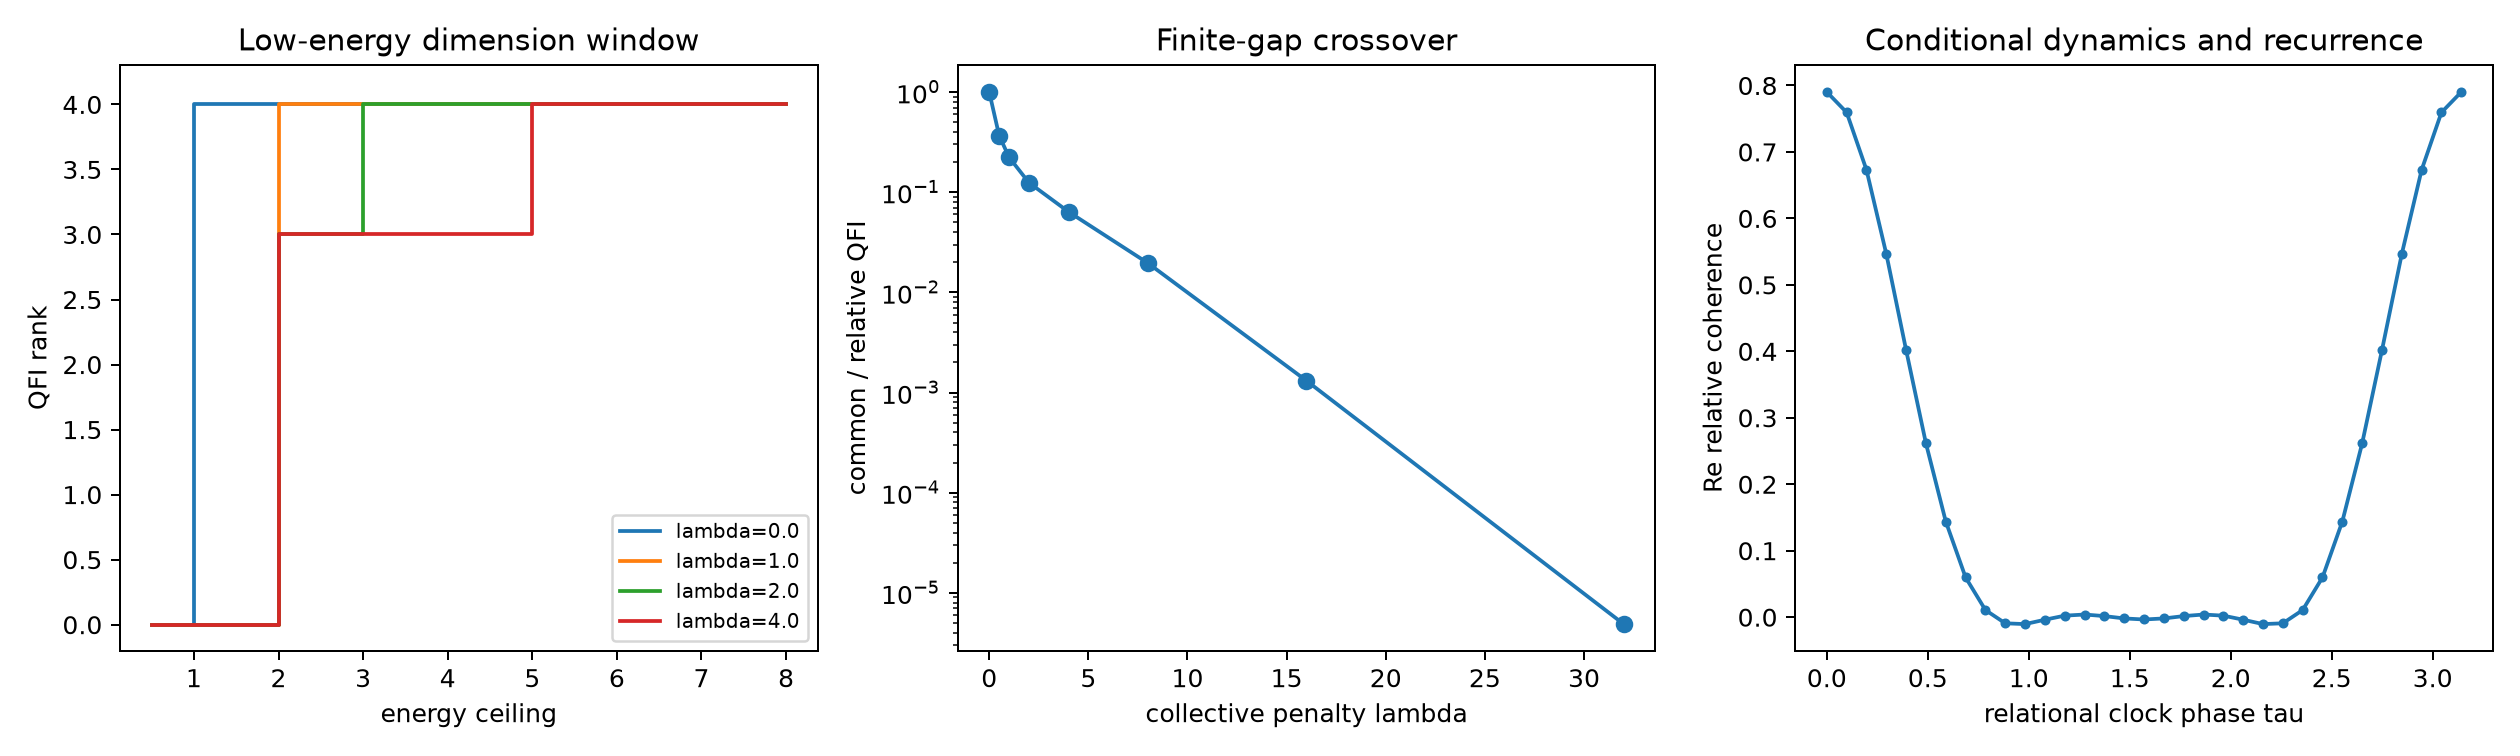
\includegraphics[width=\textwidth]{condition_atlas.png}
\caption{왼쪽: 에너지 대역에 따른 QFI rank. 가운데: 유한 집단 갭의
공통/상대 민감도 비. 오른쪽: 제약 부분공간의 조건부 상대 coherence.}
\end{figure}

\paragraph{재현성.}
수치 생성 코드는 \texttt{../src/relational\_atlas\_i01/geometry/condition\_atlas.py}, 원자료는
\texttt{../results/condition\_map.json}에 있다. NumPy의
\texttt{matrix\_rank} 허용오차는 $10^{-9}$이다. 에너지/조화 검사와
민감도 표는 결정론적이며 무작위 표본추출을 쓰지 않는다.

\begin{thebibliography}{9}
\bibitem{PW1983} D. N. Page and W. K. Wootters,
``Evolution without evolution: Dynamics described by stationary observables,''
\emph{Phys. Rev. D} \textbf{27}, 2885 (1983),
\url{https://doi.org/10.1103/PhysRevD.27.2885}.
\bibitem{PeriodicClock2026} L. Chataignier, P. A. H\"ohn,
M. P. E. Lock, and F. M. Mele,
``Relational Dynamics with Periodic Clocks,''
\emph{New Journal of Physics} \textbf{28}, 034504 (2026),
\url{https://arxiv.org/abs/2409.06479}.
\end{thebibliography}
\end{document}
